\documentclass[12pt]{article}
\usepackage{geometry}                % See geometry.pdf to learn the layout options. There are lots.
\geometry{letterpaper}                   % ... or a4paper or a5paper or ... 
%\geometry{landscape}                % Activate for for rotated page geometry
\usepackage[parfill]{parskip}    % Activate to begin paragraphs with an empty line rather than an indent
\usepackage{daves,fancyhdr,natbib,graphicx,dcolumn,amsmath,lastpage,url}
\usepackage{amsmath,amssymb,epstopdf,longtable}
\DeclareGraphicsRule{.tif}{png}{.png}{`convert #1 `dirname #1`/`basename #1 .tif`.png}
\pagestyle{fancy}
\lhead{CE 3354 -- Engineering Hydrology}
\rhead{FALL 2024}
\lfoot{ES9}
\cfoot{}
\rfoot{Page \thepage\ of \pageref{LastPage}}
\renewcommand\headrulewidth{0pt}



\begin{document}
\begin{center}
{\textbf{{ CE 3354 Engineering Hydrology} \\ {Exercise Set 9}}}
\end{center}

\section*{\small{Background}} 

The Hardin Branch study area (semester project) contains three hydrologic components that are modeled as reservoirs. These are the two SCS reservoirs and the actual highway crossing that can be approximated as a reservoir with multiple culvert outlets (beneath the highway) and a spillway (the highway elevation) approximated as a broad crested weir.

To simulate a reservoir using either level-pool routing (by-hand) or in HEC-HMS, the designer needs to construct ELEVATION-AREA and ELEVATION-DISCHARGE tables for the reservoir element. Both these tables (relationships) can be constructed from the topographic map of the study area.

Now consider the West Reservoir in the Hardin Branch analysis. Figure \ref{fig:fig1} is a portion of the topographic map that includes the SCS reservoir.

\begin{figure}[h!] %  figure placement: here, top, bottom, or page
   \centering
   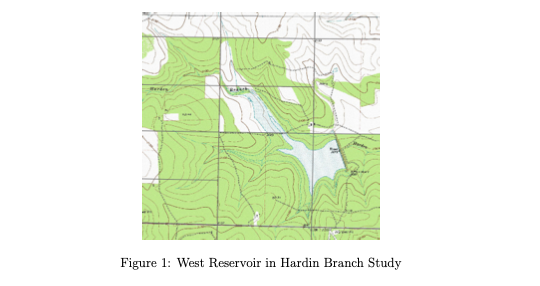
\includegraphics[width=4.0in]{fig1.png} 
   \caption{West Reservoir}
   \label{fig:fig1}
\end{figure}

The figure shows the riser elevation as 2075 feet, the spillway elevation as 2087 feet. The dam crest elevation is not explicitly labeled on the map, but 2090 feet would be a reasonable guess. Given that the spillway looks to be 50-100 feet wide, if water goes over the dam crest the designer has bigger worries than some hydrologic inaccuracy.

Suppose we choose to start a an analysis of the reservoir as empty (or just below the riser elevation). The toe (base) of the dam is about 2070 feet. Even if there is water in the reservoir it would drain slowly (hence the 7 days time to drain in the project problem statement) until the riser begins to carry flow.

\begin{figure}[h!] %  figure placement: here, top, bottom, or page
   \centering
   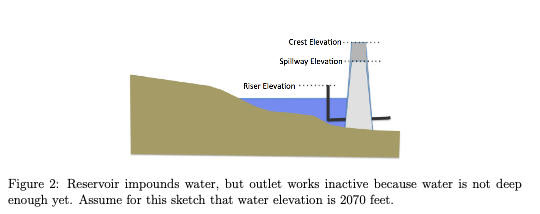
\includegraphics[width=4.0in]{fig2.png} 
   \caption{Outlet Works Schematic (dead pool elevation)}
   \label{fig:fig2}
\end{figure}

Figure \ref{fig:fig2} is an elevation view sketch of such a condition, some water is impounded, but there is no outflow because the riser pipe is not submerged and carrying any flow away from the reservoir. Typically all reservoirs leak a little so one could do some groundwater modeling to estimate the time to drain. If the reservoirs are intended to serve as stock tanks, then that’s what we want. Impoundment to some elevation so the moo cows have water to drink and poop in, but if the inflow gets too large, the flood wave that would destroy our reservoir is routed through the riser, and if the storm is really big, then the emergency spillway activates.

A typical dry-bottom detention basin design is similar, but we usually provide really small drainage structures (in addition to the riser and emergency spillway) through the toe of the dam (think small drain pipe 4-6-inches in diameter – they don’t carry much flow but will drain the reservoir slowly.)

Figure \ref{fig:fig3} is the topographic map of the pool area associated with 2070 feet (mislabeled in the figure). So this pool area is measured using AcrobatPro, Autocad, or counting squares to produce a pair of values: ELEVATION (in feet), and AREA (in Acres).

\begin{figure}[h!] %  figure placement: here, top, bottom, or page
   \centering
   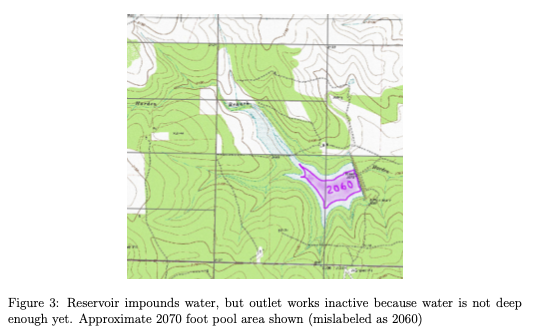
\includegraphics[width=4.0in]{fig3.png} 
   \caption{Impounded pool area schematic (pool elevation 2070 ft.)}
   \label{fig:fig3}
\end{figure}

Now as our reservoir fills, more pool area is involved as well as the outlet works begin to engage.

Figure \ref{fig:fig4} is a sketch with the pool elevation a little above the riser elevation. In this situation, pool area is determined as in the above case (different elevation of course!), and the outflow is determined using an orifice equation (or culvert equation if the pipe is horizontal).

\begin{figure}[h!] %  figure placement: here, top, bottom, or page
   \centering
   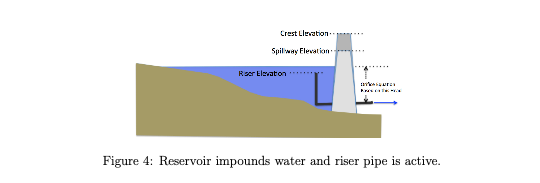
\includegraphics[width=4.0in]{fig4.png} 
   \caption{Outlet works schematic (pool elevation 2070 ft.)}
   \label{fig:fig4}
\end{figure}

Figure \ref{fig:fig5} is the topographic map of the pool area associated with 2075 feet. So this pool area is measured using AcrobatPro, Autocad, or counting squares to produce a pair of values:ELEVATION (in feet), and AREA (in Acres). AT 2075 feet the riser is just beginning to activate, so the outflow rate would be pretty small. As the reservoir further fills (from upstream inflow generated by a storm), then when the pool elevation goes above the spillway, the spillway activates (as well as the already active riser outlet).

\begin{figure}[h!] %  figure placement: here, top, bottom, or page
   \centering
   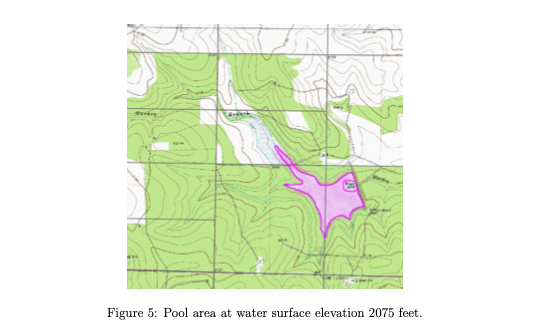
\includegraphics[width=4.0in]{fig5.png} 
   \caption{Impounded pool area schematic (pool elevation 2075 ft.)}
   \label{fig:fig5}
\end{figure}

Figure \ref{fig:fig6} is a sketch of such a situation. The head on the riser is different than the head on the spillway, hence there would be two different hydraulic equations employed to estimate discharge from the reservoir.

\begin{figure}[h!] %  figure placement: here, top, bottom, or page
   \centering
   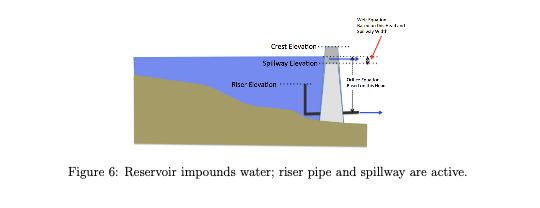
\includegraphics[width=4.0in]{fig6.png} 
   \caption{Outlet works schematic (pool elevation 2075 ft.)}
   \label{fig:fig6}
\end{figure}

Figure \ref{fig:fig7} is the topographic map of the pool area associated with 2078 feet. So this pool area is measured using AcrobatPro, Autocad, or counting squares to produce a pair of values: ELEVATION (in feet), and AREA (in Acres).

\begin{figure}[h!] %  figure placement: here, top, bottom, or page
   \centering
   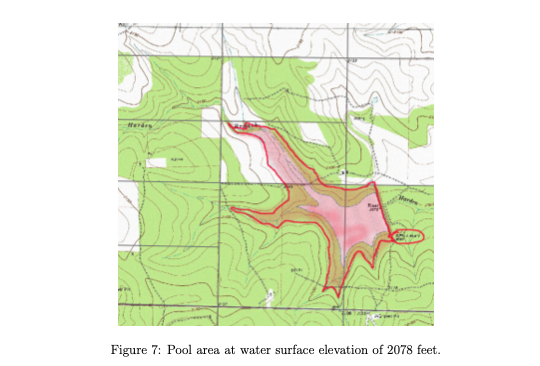
\includegraphics[width=4.0in]{fig7.png} 
   \caption{Impounded pool area schematic (pool elevation 2078 ft.)}
   \label{fig:fig7}
\end{figure}

At 2078 feet the spillway is just beginning to activate, so the outflow rate over the spillway would be pretty small, but the riser pipe has 3 feet of head above its inlet so it would be carrying substantial discharge at this point.

When we get above the top of the dam things get bad – generally we will design the spillway to pass the 100-year storm from the contributing drainage basin upstream of the dam.

\begin{figure}[h!] %  figure placement: here, top, bottom, or page
   \centering
   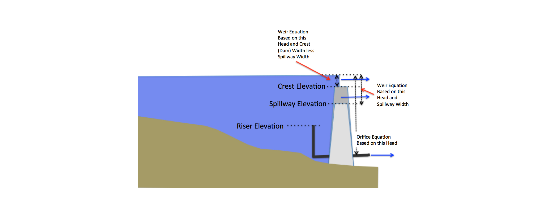
\includegraphics[width=4.0in]{fig8.png} 
   \caption{Outlet works schematic (pool elevation 2090 ft.)}
   \label{fig:fig8}
\end{figure}

Figure \ref{fig:fig8} illustrates the Darwinian case – there will be three hydraulic equations each estimating discharge for the three different parts of the outlet works. Flow over the top of the dam (less whatever width is attributed to the spillway), flow over the spillway, and flow through the riser pipe.


\begin{figure}[h!] %  figure placement: here, top, bottom, or page
   \centering
   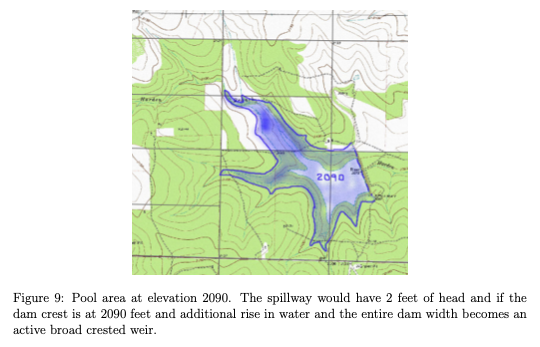
\includegraphics[width=4.0in]{fig9.png} 
   \caption{Impounded pool area schematic (pool elevation 2090 ft.)}
   \label{fig:fig9}
\end{figure}

Figure \ref{fig:fig9} is the topographic map of the pool area associated with 2090 feet. So again this pool area is measured using AcrobatPro, Autocad, or counting squares to produce a pair of values: ELEVATION (in feet), and AREA (in Acres).

Finally when the various pool areas are drawn and measured the ELEVATION-AREA table can be assembled for input later into HEC-HMS (or roll-your-own routing table). For example, the West Reservoir depicted would have a table that looks like Figure \ref{fig:fig10} which relates the pool elevation and pool area.


\begin{figure}[h!] %  figure placement: here, top, bottom, or page
   \centering
   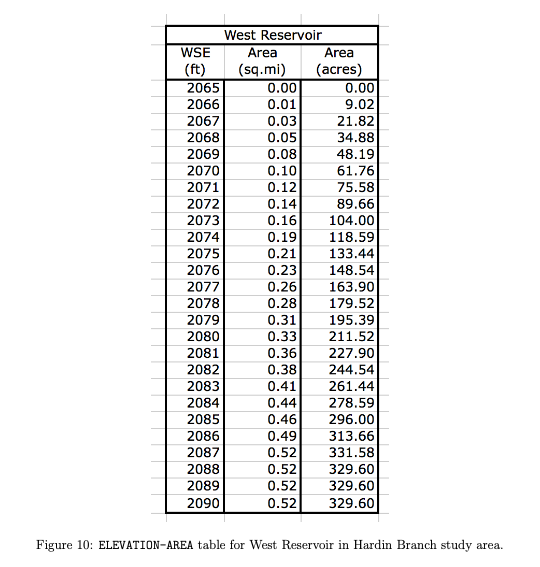
\includegraphics[width=4.0in]{fig10.png} 
   \caption{Impounded pool area schematic (pool elevation 2078 ft.)}
   \label{fig:fig10}
\end{figure}

Some of the values appear to be static, but actually reflect “rounding” that was employed in formatting the spreadsheet. The choice of using 1-foot elevation changes is analyst preference.
\clearpage

\section*{\small{Exercises}} 

\begin{enumerate}

\item Verify the ELEVATION-AREA table for the West Reservoir in the Harding Branch study area.3 You will need this table for the HEC-HMS model. Explain your choice of “bottom” elevation. Use sketches to show the relationship of elevation to different storage and outflow conditions. Plot the area-elevation curve (area is on the x-axis). Indicate on the plot the elevations where outlet works would activate.

\item Construct an ELEVATION-AREA table for the North Reservoir in the Harding Branch study area. You will need this table for the HEC-HMS model. Explain your choice of “bottom” elevation. Use sketches to show the relationship of elevation to different storage and outflow conditions. Plot the area-elevation curve (area is on the x-axis). Indicate on the plot the elevations where outlet works would activate.

\item Construct an ELEVATION-AREA table for the US-87 highway crossing in the Harding Branch study area. You will need this table for the HEC-HMS model. Explain your choice of “bottom” elevation, and spillway elevation. Use sketches to show the relationship of elevation to different storage and outflow conditions. Plot the area-elevation curve for the crossing structure (x-axis is area). Indicate on the plot the elevations where the culverts would become active (carry flow) and when the road surface (spillway) would become active.

\end{enumerate}

\end{document}  